%%%% 1. DOCUMENTCLASS %%%%
\documentclass[journal=tosc,final]{iacrtrans}
%%%% NOTES:
% - Change "journal=tosc" to "journal=tches" if needed
% - Change "submission" to "final" for final version
% - Add "spthm" for LNCS-like theorems


%%%% 2. PACKAGES %%%%
\usepackage[left, pagewise, edtable]{lineno}

\usepackage{graphicx}
\usepackage{framed} 
\usepackage{xcolor}
\usepackage{tcolorbox}
\usepackage{xcolor} 
\colorlet{shadecolor}{gray!25}
\definecolor{mshadecolor}{rgb}{0.7421875,0.7421875,0.7421875}
\setlength{\OuterFrameSep}{10pt}
%%%% 3. AUTHOR, INSTITUTE %%%%
\author{Moritz Rupp}
\institute{
  Hochschule Albstadt-Sigmaringen, Albstadt, Germany, \email{ruppmori@hs-albsig.de}
  
}
%%%% NOTES:
% - We need a city name for indexation purpose, even if it is redundant
%   (eg: University of Atlantis, Atlantis, Atlantis)
% - \inst{} can be omitted if there is a single institute,
%   or exactly one institute per author


%%%% 4. TITLE %%%%
\title{Fuzzing Methods}

\author{Moritz Rupp}
%%%% NOTES:
% - If the title is too long, or includes special macro, please
%   provide a "running title" as optional argument: \title[Short]{Long}
% - You can provide an optional subtitle with \subtitle.

\begin{document}

\maketitle
\author


%%% 5. KEYWORDS %%%%
\keywords{Offensives Security \and Fuzzing \and Brute-Forcing \and It-Security \and Testing }


%%%% 6. ABSTRACT %%%%
\begin{abstract}
Modern Softwares has become increasingly more complex. This is connected with growing nummbers of security bugs and cyberattacks[1]. Software testing tries to oppose that development. Fuzzing is a dynamic automated way of testing systems and sees growing usage among security profesionals. It has gained growing attention after several zero day vulnerabilitys have been found with this approach. This paper examines different methods to use this technology. 
\end{abstract}

%%%% 7. PAPER CONTENT %%%%
\section{Introduction}
Development of any kind has always come with bugs, errors and unintentionally behaviour. Software is no exception. Increasingly complex programs and growing technology stacks contribute to this problem. On top of that, finished components are often continuously integrated. As a result, it becomes ever more difficult to predict final program behaviour. This yields in risks, particular if an application is processing external data input. If not handled correctly it can pose security vulnerabilitys or data breaches.

The bigger a programm gets, more often such unwanted appearances occur. A field in which this is most noticable is web-development. Whereas 15 years ago, most websites were built on top of a view technologys, modern web-applications often use several framework with huge amounts of dependencys. This lead to an increasing amount of security bugs[2]. Different approaches in software testing tries to oppose that development.

Back when software was relativly simple and free of dependencys, manuel testing was the state of play. That included code reviews and manuel checks for potentiel exploitation. This was time consuming and needed experts for every specific application. Therefore static analyis was quickly adapted. This contained new techniques such as pattern search with a control flow graph, data dependency graph and data flow analysis[3]. When software grew even more in complexity, security researchers needed a more scalable approach. Hence dynamic analyis was implemented. This method tries to understand software behaviour by testing and evaluating the target system while it is running. 

Fuzz-testing is the cutting edge of this technique and will be explored in this paper. A particular emphasis will be led on the different methods used in fuzzing. 
At first we will examine the basic concepts and functionality of the general approach. On top of that different methods in Fuzzing will be explored. That expresses itself in how certain functionalitys of the fuzzing application are executed. This section will be the main focus of the paper. Following we will also cover practical usage by showcasing different tools and a concrete example. 

As a final point we will have a conclusion in which we provide a summary and an assessment of the pros and cons of Fuzz-testing. 
\newpage
\section{Fuzzing background}
Fuzz testing or fuzzing is a method of testing software to detect security holes in applications, operating systems, and networks. It involves flooding their input interfaces with random data, called fuzz, to make them crash or trigger unexpected programm behaviour. Furthermore the computation results are monitered and reported, all in an automated way. Fuzzing has become increasingly more relevant among security researchers and is used by almost all big tech companys for penetration testing[4]. Tech leaders find more than 80 of their bugs by using different fuzzing Methods[5]. Google for example  has found over 15 thousend errors in their browser projekt chrome[6]. Microsoft used dynamic analysis to test one of their flagship projects 'office' and found nearly 2000 bugs using the fuzzing tool afl[7]. Also open source project such linux use Fuzzing methods on a great scale. Many security bugs within the Linux Kernel have been found this way[8].\\
Generally a distinction can be made on how fuzzing is executed on a specific interface. Depending on the application or infrastructure of the target system, different types of fuzzers can be used. Application Fuzzing will approach a system by testing functionalitys such as buttons, input fields or command line parameters. File format fuzzing tries to generate corrupted files and feed them to the corresponding target for processing. Other types of fuzzing targets include Protocol Fuzzing and Network fuzzing.\\
In addition more distinction can be made on how the fuzzing inputs or test cases are generated. There are two approaches. Mutation based Fuzzers alter existing data samples to create new test cases.
Generation based fuzzers will create test cases from scratch based on protocoll knowledge. 
Both methods have pro and cons and will be covered in more detail later on.

\section{Functionality}
This section will provide a perspective on the basic concept of Fuzzing.

Regardless of the specific implementation, the core process of all fuzzers remains the same. First the target interface has to be identified. Relevant are all interfaces that allow external data input. This ranges from network sockets, user-input on a website, to linux binarys et cetera. Specifically interesting are interfaces that are reachable by unpriviliged users. The act of finding those target interfaces highly depends on the tested application and could include things like code reviews or portscanning. 


Based on the findings, the fuzzer input can now be generated. This is one main task of the actual fuzz-engine. In the most basic case, it will generate pseudo random inputs based of the given seed. The seed could contain anything that makes sense in the context of the expected data[9]. Essentially a snapshoot of valid inputs for the target system. This will be mostly combinations of strings and intergers. 

Following the test cases can be passed to the  target system. Depending on the identfied interfaces, different transfer methods are used. This could involve HTTP Requests, tcp sockets or simply files or input parameters for a programm. While the Fuzz-engine is sending the generated inputs, the target system has to be monitered to track how the testcases effect the system behaviour. Monitering and tracking can be achieved with different approaches. A convinient but not always available case are logging functions of the target system. They can be simply read out during or after the fuzzing process. If the target is lacking such functionalitys they first have to be implemented. 

More features are feedback instrumentations. Those are compile time binarys that are inserted into the target code to track and tell the fuzzer which parts of the internal programmflow is effected and has already been covered. This ensures to establish a correlation between test cases and programm behaviour. The Feedback gets send back to the fuzzing-engine and can be read out or reprocessed[10].
\newpage

\noindent Figure 1 provides an overview of a basic mutation based fuzzing implementation. The Fuzzer as seen between the Seed and the target system includes a mutation engine and genetic algorithms. The Fuzzing process can now lapse as follows.\\
The Seed streams valid inputs to the fuzzer that will modifiy these with the help of the mutation engine. Following the mutated inputs gets send to the target system in which feedback instrumentations listen for exceptions, log them and provide feedback to the fuzzer. Based on that genetic algorithms produce further inputs.

Once the fuzzing process has endet, it is now possible to analyse and minimize the findings. This includes to determine if a tracked exeption could actually cause a vulnability or even an exploit. Furthermore these assessments are rated. This is done by ranking frameworks like the common vulnability scoring system(CVSS)[11]. Finally all relevant informations are summed up, reported and passed to the corresponding responsible. 
\begin{shaded}

\begin{center}
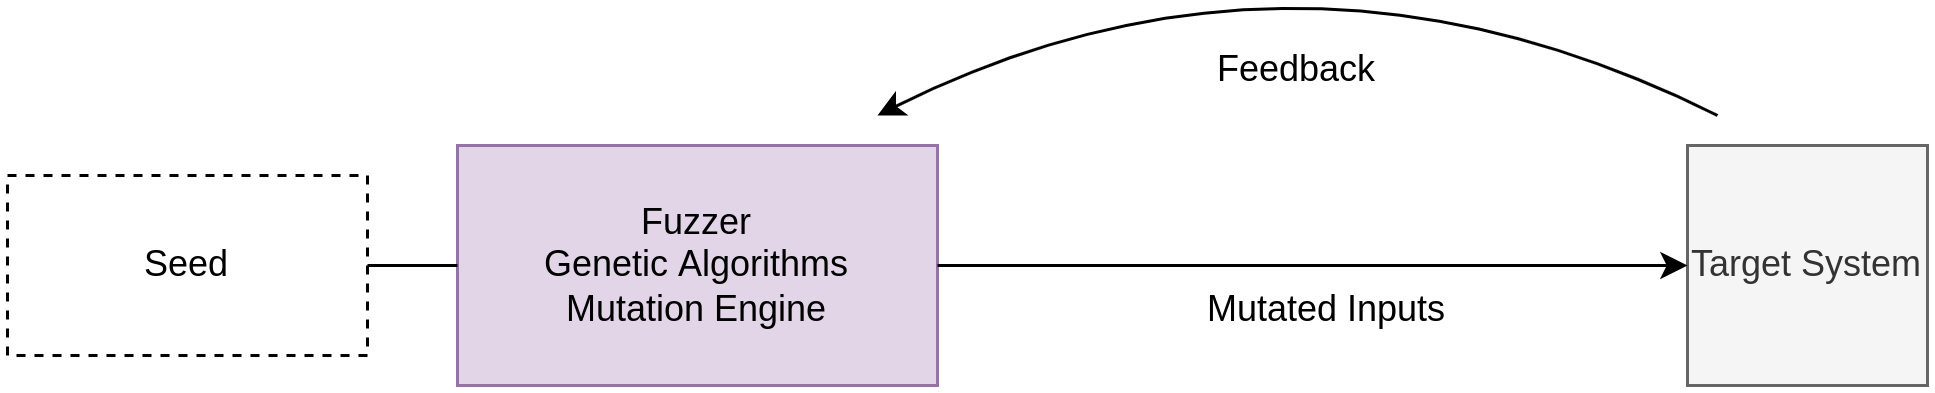
\includegraphics[scale=0.2]{../final2.png}

\vspace{2mm} Figure 1: Basic Fuzzing application
\end{center}
\end{shaded}


\section{Fuzzing Methods}
Due to the huge landscape of applications, infrastructures and use cases, enourmes classifications exist around fuzzing. 

In this section we will further examine the different methods used to generate the fuzzing input, like random, mutation and generation based fuzzing. Afterwards we will also cover different types of target focused fuzzers such as application or file format fuzzing et cetera. 
\subsection{Random fuzzing}
When fuzzing was invented in 1988 by Professor Barton P. Miller at the University of wisconsin, random fuzzing was the very first approach[12].

When Miller held a lecture remotely via a telephone connection, a thunderstorm caused electrical disturbances in the telephoneline. This resulted in garbled transmissions. Based on these random occuranced, Miller stated that bad input  could be used to crash other systems. He and his students applied this observation on different unix utilites their where using at that time. They remarked that  more than 30\% of the tested programms where vulnerable to bad input[13]. 

Initally they simply manuelly passed pseudo random inputs to these programms. Later on miller made a programming assigment to his students, that stated to automate this task. The very first fuzzer was born. The basic principle still holds up today. 

Random fuzzers will simply generate inputs by randomly concatenate characters that are provided in a seed. The method is mainly used for black box testing, since in there input formats are mostly unknown. A clear downside are the huge amounts of invalid inputs such a fuzzer will produce. 

Most of the generated test cases are getting rejected by the parser of the target programm. Hence random fuzzers are often used to test parser applications.

Another usecase are to fuzz strings of programm parameters. They barely follow any specific structure and are therefore an ideal target for random bazzed fuzzers. 
\subsection{Mutation based fuzzing}
As we already know, this method will simply alter already existing data. This can be based of available information in case the target inputs are known. Otherwise it is first neccecarry to record valid inputs. This can be achieved via proxys that will record communication or interaction patterns. These valid inputs can then be mutated, either in a completly random manner or after fixed patterns. Figure 2 provides a mutation based implementation in pseudo code. 

\begin{center}
\begin{shaded}
\begin{internallinenumbers}
\begin{verbatim}

seed = "https://www.hs-albsig.de/such?tx\_solr[q]=\\"
Fuzzer = MutationFuzzer(seed=seed)
Fuzzer.mutate for i in alphabet -->
"https://wGw.h2-albsig.re/sLh?tx\_soslr[qx=?\"
"htSpK://wwl.hs-albsisag.de/such?tx\_solr[s]a\\"
"htSps://o?w.h_s-lbsig.de/such?tx\_solr[q]=\p"
"h?tpIl//wsw.hs-albswgqde/such?tx\_solr[q]=q\"
"https://www.hs-albsig.de/such?tx\_solr[q]=\\"
\end{verbatim}
\end{internallinenumbers}
\vspace{2mm} Figure 2: Mutated Fuzzing outputs
\end{shaded}
\end{center}
At first, in line 1 the seed is determined. Following a Fuzzer object is applied and the seed is passed(see line 2). Then we call the fuzzer method to mutate the given inputs without setting up any fixed patterns. This results in several mutated urls. The inner procedure is simple.

The fuzzer engine will take a random index of the seed in the range of the string length. The index value will then be flipped.  Here we instantly see why mutation based fuzzers are often called 'dumb fuzzers'. 
Most of the generated outputs are invalid urls, and will be rejected by the parser of the target system. In fact several of the generated urls will never reach our inital target, the webserver. This implementation will moreover fuzz the url-parser than the http-server.
Therefore it is neccecarry to be very patience about which part of valid inputs should get passed to the seed to be fuzzed. 

In this concrette example the right approach would be to setup a  static corpus and only mutate the string of the file path and parameters. 
These can then be combined and send out.
\begin{center}
\begin{shaded}
\begin{verbatim}
static = https://www.hs-albsig.de/  seed = "suche/?tx\_solr[q]=\\"
\end{verbatim}
\vspace{2mm} Figure 3: Mutated Fuzzing outputs
\end{shaded}
\end{center}
Even more precision can be achived by providing multiple seeds that represent different parts of the valid format. A simple function can then receive mutation of those seeds and concatenate them within the expected format.

\newpage
\subsection{Generation based fuzzing}
In Generation-Based fuzzing new data is defined based on the expected input of the target specification. Hence knowledge of the system under test is mandatory. It is neccecarry to have a well understanding of the input format, since test cases are generated completly from scratch.  
\subsection{Application Fuzzing}

\subsection{Protocoll Fuzzing}
\subsection{File format Fuzzing}
\subsection{Network Fuzzing}
\newpage
\section{Tooling}
Hundrets of fuzzing tools are availabls. Like wfzuu, afl and zfuzz etc..
\subsection{Practical example}
We will fuzz a webserver with afl\dots
\section{Conclusion}




\section{References}
[1] \textbf{Aimee O'Driscoll}(2022), 25+ cyber security vulnerability statistics and facts of 2022, https://www.comparitech.com/blog/information-security/cybersecurity-vulnerability-statistics/\\
\\
\noindent[2] \textbf{Emilio Granado Franco}(2022),  Global Risks Report 2022, Chapter 3. Digital Dependencies and Cyber Vulnerabilities\\

\noindent[3] \textbf{Chess, B. and McGraw, G.}(2004), Static analysis for security, IEEE Security \& Privacy, 10.1109/MSP.2004.111
\\


\noindent[4] \textbf{Li, Jun and Zhao, Bodong and Zhang, Chao}(2018),     Fuzzing: a survey, SpringerOpen
\\

\noindent [5] \textbf{Sergej Dechand}(2020), Introduction and fuzzing 101 @Fuzzconn Europe 2020, CodeIntelligence, https://www.youtube.com/watch?v=7AdzrXbUew0
\\

\noindent [6] \textbf{Liam Tung}(2019),  Google: We've open-sourced ClusterFuzz tool that found 16,000 bugs in Chrome, https://www.zdnet.com/article/google-weve-open-sourced-clusterfuzz-tool-that-found-16000-bugs-in-chrome/
\\

\noindent [7] \textbf{Sergej Dechand}(2020), Introduction and fuzzing 101 @Fuzzconn Europe 2020, CodeIntelligence, https://www.youtube.com/watch?v=7AdzrXbUew0
\\

\noindent[8] \textbf{Jonathan Reimer}(2020), 5 CVEs Found With Feedback-Based Fuzzing, https://www.code-intelligence.com/blog/5-cves-found-with-feedback-based-fuzzing
\\

\noindent[9] \textbf{Li, Jun and Zhao, Bodong and Zhang, Chao}(2018),     Fuzzing: a survey, SpringerOpen
\\


\noindent[10] \textbf{Cornelius Aschermann}(2020), Algorithmic Improvements for
Feedback-Driven Fuzzing, SpringerOpen
\\

\noindent[11] \textbf{NIST}(2019), Vulnerability Metrics, https://nvd.nist.gov/vuln-metrics/cvss
\\

\noindent[12] \textbf{Parul Garg}(2012), Fuzzing: Mutation vs. generation, https://resources.infosecinstitute.com/topic/fuzzing-mutation-vs-generation/
\\

\noindent[13] \textbf{Andreas Zeller}(2022), Fuzzing: Breaking things with random inputs, https://www.youtube.com/watch?v=YjO1pIx7wS4/
\\
\end{document}
